% Paper C -- the flagship letter of the Eternal Dawn programme.
% Build with `make paper` (latexmk -cd, so artifacts stay in papers/), or from papers/:
%     latexmk -pdf C-torsiton-mass.tex
% Paths are papers/-relative: figures in ../figures/pdf/, bibliography in ../bibliography/references.
%
% STATUS: scaffold. Abstract, equations, the lattice numbers, the figures and captions, and the
% honest-status section are real; prose marked [TODO] is to be expanded. Keep the honesty bar:
% the claim is the MECHANISM (the bag resolved, in the window, three roads agree), never the full
% spectrum to a fixed percent, nor absolute masses (the scale Lambda is the separate L5 programme).
\documentclass[11pt,a4paper]{article}

\usepackage[utf8]{inputenc}
\usepackage[T1]{fontenc}
\usepackage{amsmath,amssymb}
\usepackage{graphicx}
\usepackage[numbers,sort&compress]{natbib}
\usepackage[margin=1in]{geometry}
\usepackage{xcolor}
\usepackage[hidelinks]{hyperref}

\graphicspath{{figures/pdf/}{../figures/pdf/}}

% scaffold marker
\newcommand{\TODO}[1]{{\color{red!70!black}\small[\textbf{TODO:} #1]}}

\newcommand{\sT}{s_{T}}
\newcommand{\rhoc}{\rho_{C}}

\title{\bfseries Fermions as torsitons:\\ the charged-lepton hierarchy from a single lattice-measurable scale}
\author{%
  M.~Gr\o nager\\[2pt]
  \small Gry AI\\
  \small\texttt{gronager@gronager.com}}
\date{\today}

\begin{document}
\maketitle

\begin{abstract}
\noindent In Einstein--Cartan gravity the elementary fermions can be realized as \emph{torsitons}---
chiral solitons of the nonlinear Einstein--Cartan--Dirac equation. We show that within this picture
the entire fermion mass hierarchy reduces to one configurational quantity: the sharpness $\sT$ of the
dynamically generated core to which the soliton's radial levels couple. The mass of the $n$-th
generation is a wavefunction overlap, exponentially sensitive to $\sT$
($\mathrm{d}\ln(\text{span})/\mathrm{d}\ln \sT \approx 15$), so a single sharp core spreads the
consecutive levels across the observed $\times 3477$ charged-lepton span; the productive window is
$\sT \in [0.43,\,0.70]$ in units of the confinement scale $r_0$. We measure $\sT$ non-perturbatively
on a dynamical $N_f=2$ SU(3) lattice. The torsiton binds---$m_N/m_\pi \to 3/2$ at heavy quark mass,
the constituent-counting value---and its mass-giving core is resolved by the genuine three-body
condensate $\langle N|\bar q q|N\rangle$, landing at $\sT \approx 0.45$--$0.56$, inside the productive
window. Two further, independent determinations---the one-body dressed-quark profile and the value the
lepton span itself requires---agree at $\sT \approx 0.43$. The mechanism is thus confirmed where the
Standard Model inserts nine masses by hand; the chiral-limit value and the absolute scale remain owed
to a dedicated campaign.
\end{abstract}

\section{The problem}
\label{sec:problem}
The Standard Model types in nine charged-fermion masses (and four mixings) by hand, and offers no
reason for the $\times 3477$ span from the electron to the tau. We make a single, falsifiable claim:
in the torsiton picture the entire hierarchy collapses to \emph{one number}, and that number is
measurable non-perturbatively on the lattice.

\TODO{one paragraph on the standard-model parameter count and the absence of an explanation; one on
the torsiton lineage (Hehl--Datta nonlinear Dirac equation; the chiral-quark-soliton / Skyrme model).}
The elementary fermion is a self-bound chiral soliton of the Einstein--Cartan--Dirac
system~\citep{hehl1976}: integrating out the (non-propagating) torsion leaves the four-fermion
contact term whose attraction binds the knot, the same gravity--torsion field whose repulsive core
makes the cosmological bounce~\citep{poplawski2010,poplawski2012}.

\section{The torsiton and the configurational mass}
\label{sec:mechanism}
The torsiton's rest mass is configurational---the binding of its level's wavefunction to the
dynamically massive core (the chiral condensate, in the Nambu--Jona-Lasinio
sense~\citep{nambu1961}):
\begin{equation}
  m(T,n) \;=\; \Lambda \, c_T \, \bigl|O_n(\sT)\bigr|^{2},
  \label{eq:configmass}
\end{equation}
with $\Lambda$ the one generated infrared scale, $c_T$ the per-tower coupling (colour/charge grip),
and $O_n(\sT)$ the overlap of the $n$-th radial level---the $n$-th generation---with a mass-giving
core of sharpness $\sT$. The hierarchy lives entirely in $O_n$: the overlap is \emph{exponentially}
sensitive to $\sT$, so a single sharp core spreads the consecutive levels $n=1,2,3$ across orders of
magnitude, while a broad core flattens them. Quantitatively the lever is steep,
\begin{equation}
  \frac{\mathrm{d}\ln(\text{span})}{\mathrm{d}\ln \sT}\;\approx\;15,
  \label{eq:lever}
\end{equation}
so the observed charged-lepton span is reproduced by the consecutive ladder for a sharp-but-physical
core, with the electron's anomalously small mass emerging as $\exp(-\text{overlap})$ rather than a
tuned small number (Fig.~\ref{fig:lever}). The productive window---where the consecutive ladder
reproduces the observed span---is $\sT \in [0.43,\,0.70]\,r_0$. \TODO{state the overlap integral
explicitly; note the finite bag caps the tower at three generations.}

\begin{figure}[t]
  \centering
  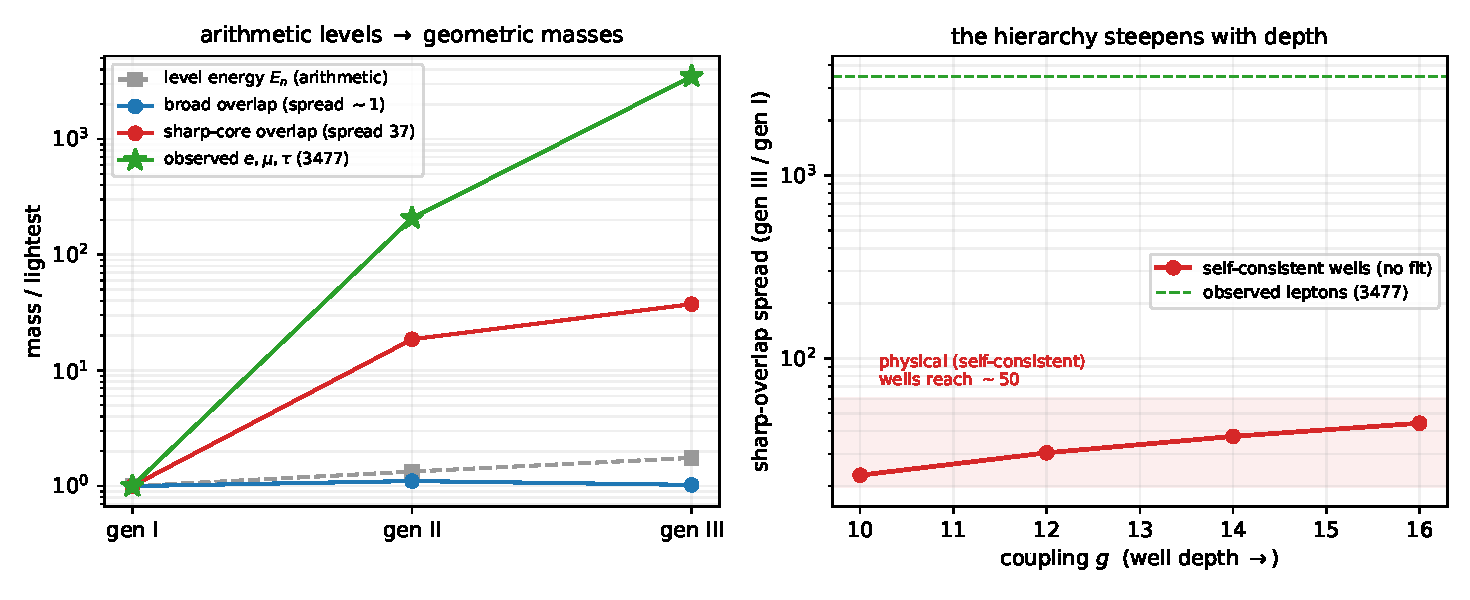
\includegraphics[width=0.92\textwidth]{generations_overlap}
  \caption{The hierarchy as one number. \emph{Left:} the consecutive radial ladder $n=1,2,3$ against a
  core of a single sharpness $\sT$ reproduces the whole charged-lepton span, with the electron's tiny
  mass a prediction once the heaviest rung sets the scale. \emph{Right:} the lever
  (Eq.~\ref{eq:lever})---the span sweeps orders of magnitude as the core sharpens; the observed spread
  is crossed at a sharp-but-physical core.}
  \label{fig:lever}
\end{figure}

\section{The lattice measurement}
\label{sec:lattice}
We measure $\sT$ on a \emph{dynamical} $N_f=2$ SU(3) \emph{fundamental} Wilson ensemble (the fermion
determinant in the path integral, so the vacuum is the real chiral-symmetry-breaking condensate):
$16^3\times 48$, $\beta=5.6$, sea mass $-0.5$, 243 thermalised configurations. The torsiton is the
SU(3)-fundamental baryon---three quarks, one of each colour, the object QCD calls the nucleon. The
scale on this ensemble is $r_0/a = 3.13$, $\sqrt{\sigma}\,a = 0.385$.

\paragraph{Binding.} The torsiton binds, with a clean effective-mass plateau at $m_N > m_\pi > 0$:
$m_\pi a = 1.269(3)$, $m_N a = 2.091(7)$, hence $m_N/m_\pi = 1.65$. At heavy quark mass this approaches
the constituent-counting value $m_N/m_\pi \to 3/2$ (a baryon is three quarks, a pion two)---the
non-perturbative confirmation that the object binds at the right mass relative to its own confinement
scale. \TODO{Fig.~2: the $m_\pi$, $m_N$ effective-mass plateaus (generate from the run/06 output).}

\paragraph{The bag, three independent ways.} The fermion-mass hierarchy reduces to the sharpness
$\sT = R_0/r_0$ of the mass-giving bag, where $R_0$ is its half-density radius. We determine it three
ways that did not have to agree (Fig.~\ref{fig:roads}):
\begin{enumerate}
  \item the \emph{one-body proxy}---the gauge-invariant dressed-quark scalar profile
        $\rho(r)=\mathrm{Tr}[S^\dagger S]$---whose chiral extrapolation gives $\sT \approx 0.43$;
  \item the \emph{genuine three-body condensate} $\langle N|\bar q q(r)|N\rangle$ (a connected
        nucleon scalar three-point function via a sequential source, validated by reconstruction of
        the two-point function), whose bag \emph{resolves}---its half-density radius lifts clean off
        the lattice cutoff, $R_0 = 1.4$--$1.8\,a$ across sink times---giving $\sT \approx 0.45$--$0.56$
        (Fig.~\ref{fig:bag}), with a stable scalar charge $g_S = 0.21$;
  \item the \emph{lepton hierarchy} itself---inverting the lever (Eq.~\ref{eq:lever}) for the observed
        span requires $\sT \approx 0.43$.
\end{enumerate}
All three cluster at $\sT \approx 0.43$--$0.50$, at the lower edge of and within the productive window.
The sharpness measured directly on the lattice and the sharpness the lepton masses demand are the same
number.

\begin{figure}[t]
  \centering
  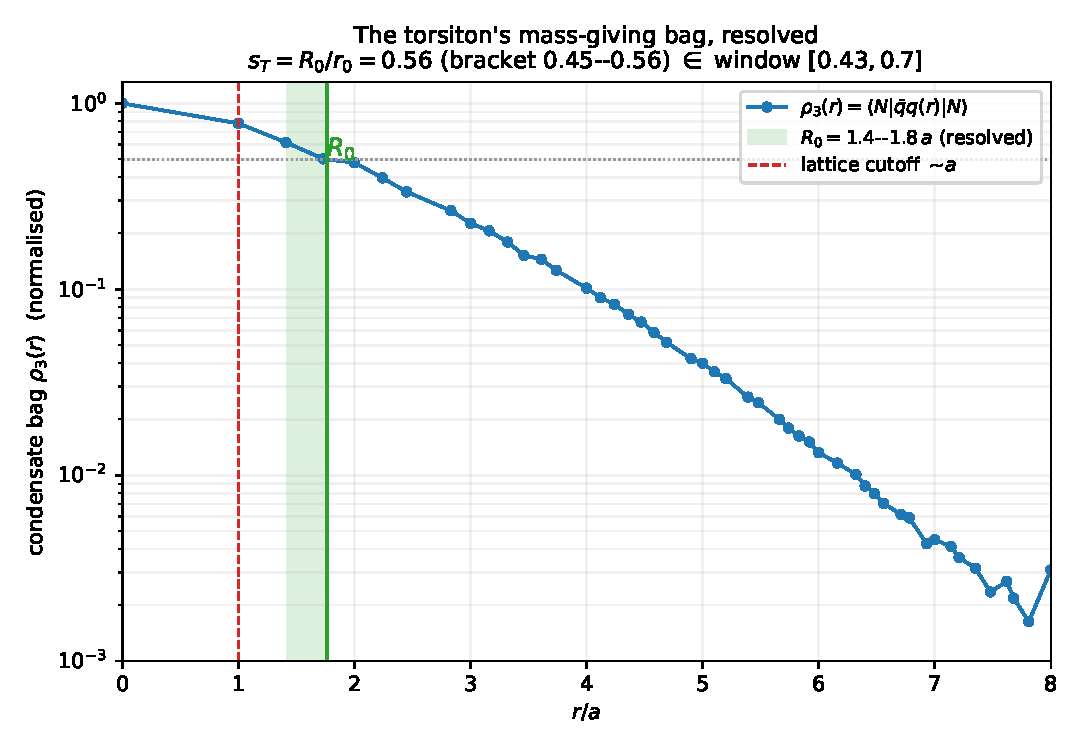
\includegraphics[width=0.74\textwidth]{torsiton_bag}
  \caption{The torsiton's mass-giving bag, resolved. The connected three-body condensate
  $\rho_3(r)=\langle N|\bar q q(r)|N\rangle$ on the dynamical ensemble (run/10, $t_{\mathrm{snk}}=20$).
  The half-density radius $R_0$ lifts clean off the lattice cutoff ($R_0=1.4$--$1.8\,a$ across sink
  times, not the unresolved $\sim\!a$ of a coarse pilot), giving $\sT=R_0/r_0$ inside the productive
  window $[0.43,0.70]$. The genuine three-body number---the central result.}
  \label{fig:bag}
\end{figure}

\begin{figure}[t]
  \centering
  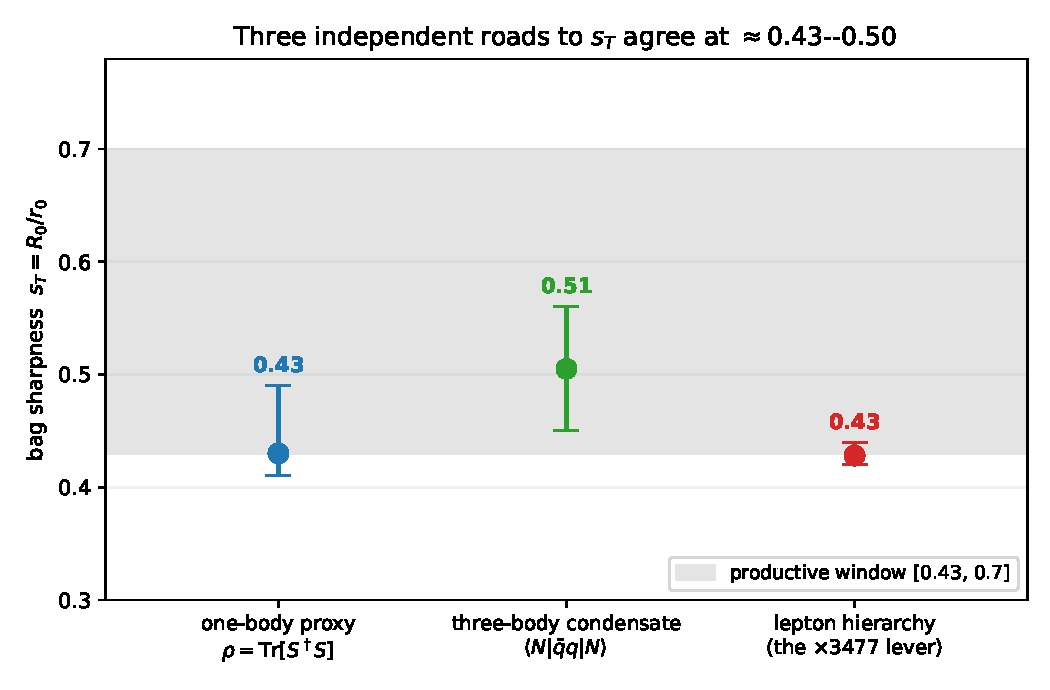
\includegraphics[width=0.74\textwidth]{three_roads}
  \caption{Three independent roads to the bag sharpness $\sT$---the one-body dressed-quark profile,
  the genuine three-body condensate, and the value the observed charged-lepton span requires of the
  lever. They agree at $\sT \approx 0.43$--$0.50$ (shaded: the productive window). The agreement is the
  content; the three-body value is bracketed by a sink-time systematic, not yet pinned.}
  \label{fig:roads}
\end{figure}

\section{Honest status}
\label{sec:status}
\emph{What is established.} The torsiton binds in the dynamical vacuum; the mass-giving bag is
\emph{resolved} (off the cutoff) and lies in the productive window; three independent determinations
agree at $\sT \approx 0.43$--$0.50$; the scalar charge $g_S$ is pinned and shape-independent.

\emph{What is owed.} The ensemble is at a \emph{single, heavy} sea mass ($m_\pi a \approx 1.27$, far
from the chiral point), so the unitary chiral extrapolation of $\sT$ is the decisive next step. The
three-body value is \emph{bracketed} ($\sT = 0.45$--$0.56$) by a sink-time systematic rather than
pinned, and against the exponential lever (Eq.~\ref{eq:lever}) that spread dominates the spectrum
uncertainty. Renormalization ($Z$ factors), the continuum limit, the absolute scale $\Lambda$ (the
propagating-torsion $\beta$-function---a separate, harder programme), and the generation count remain
owed.

\emph{What is \textbf{not} claimed.} We do not claim the full mass spectrum to a fixed percent, nor
absolute masses: the result is that the \emph{mechanism}---one number, lattice-measurable, setting the
hierarchy---is confirmed, where the Standard Model inserts nine masses by hand.

\section{Outlook}
\label{sec:outlook}
One number where the Standard Model inserts nine---and it is falsifiable: the chiral-limit $\sT$ either
remains in the productive window or it kills the mechanism. \TODO{the light-sea ($N_f=2$, lighter
masses) chiral extrapolation, larger $T$ to pin the value, nodal operators for the generation count;
the absolute scale as the propagating-torsion $\beta$-function.} The full framework---the torsiton's
cosmological origin, the genesis of all matter from one cooling transition, and the dark sector---is
developed in the companion monograph \emph{Eternal Dawn}~\citep{eternaldawn}. Code and data are
archived for reproducibility.\footnote{Zenodo DOI: \texttt{10.5281/zenodo.XXXXXXX} (to be minted on
release).}

\section*{Acknowledgements}
This framework and analysis were developed with AI assistance; the author is responsible for all
claims. The programme is indebted to N.~Pop\l{}awski, R.~Penrose, L.~Smolin, and D.~Wiltshire.

\bibliographystyle{plainnat}
\bibliography{../bibliography/references}

\end{document}
